\documentclass[a4paper,12pt]{scrartcl}

% Title page
\usepackage{authblk}

% General style
\usepackage{fontspec}
\setmainfont[BoldFont = GenBasB.ttf]{Gentium Plus}
\setsansfont{DejaVu Sans}
\usepackage{newunicodechar}
\newunicodechar{→}{\fontspec{Gentium Plus}→}

% Formulas
\usepackage{amsmath}
\usepackage{amssymb}

% Internal references
\usepackage[titletoc,title]{appendix}
\usepackage{hyperref}
\usepackage[capitalize]{cleveref}
\Crefname{appsec}{Appendix}{Appendices}
\crefname{appsec}{appendix}{appendices}

% Draft style
\usepackage{setspace}
\setstretch{1.5}
\usepackage[top=2.5cm, bottom=2.5cm, left=2.2cm, right=3.5cm]{geometry}
\usepackage{lineno} 

% Figures
\usepackage{subcaption}
\usepackage[font=small,labelfont=it]{caption}
\usepackage{graphicx}
\usepackage{tikz}
\usetikzlibrary{arrows}
\usetikzlibrary{arrows.meta}
\usetikzlibrary{decorations.pathreplacing}
\usetikzlibrary{bayesnet}
\usepackage[linguistics,edges]{forest}
\usepackage{rotating}

% Bibliography
\usepackage[backend=biber,
            bibstyle=biblatex-sp-unified,
            citestyle=sp-authoryear-comp,
            maxcitenames=2,url=false,
            maxbibnames=99]{biblatex}
\renewcommand*{\bibfont}{\small}
\addbibresource{library.bib}

\renewbibmacro*{doi+eprint+url}{%
  \printfield{doi}%
  \newunit\newblock%
  \iftoggle{bbx:eprint}{%
    \usebibmacro{eprint}%
  }{}%
  \newunit\newblock%
  \iffieldundef{doi}{%
    \usebibmacro{url+urldate}}%
  {}%
}

\newcommand{\glot}[2]{#1 {\scriptsize{[\texttt{\hyperlink{https://glottolog.org/resource/languoid/id/#2}{#2}}]}}}

% Code inclusion with syntax highlighting
\usepackage{minted}
\setminted{fontsize=\tiny,baselinestretch=0.9}

\title{Burst Clock}
\date{\today}
\author[1]{Nico Neureiter}
\author[1]{Gereon A. Kaiping}
\affil[1]{Geographic Information Science Center, Universität Zürich, CH}

\begin{document}
\maketitle
\begin{abstract}
When a language splits into different speaker communities, the speed of
language change increases. \Textcite{atkinson2008languages} showed that a
significant proportion of up to a third of lexical disparity can be attributed
to the splitting events, potentially arising from linguistic founder effects or
the exaggeration of language differences to mark social boundaries. Given the
prevalence with which phylogenetic models in linguistics are used to date
language families, it is surprising that this result has not found its way back
into the clock models used in phylogenetic inferences, which tend to focus
instead on per-branch variation \parencite{}. Here, we develop a simple
extension to the Strict Clock model \parencite{} in BEAST2 \parencite{} to
account for bursts at language splits. We use simulation studies and also fit
the new model to four major language families of the world –~Austronesian,
Bantu, Indo-European, and Sino-Tibetan~– and find that the Burst Clock fits the
data better than either a Strict Clock or an Uncorrelated Relaxed Clock, and on
average a binary split is associated with XXX lexical changes in the basic
vocabulary. This is equivalent to the amount of lexical change a language
accumulates in about 100 years of independent evolution. Similar bursts of evolution
occur also at initial niche settlement in biology, so the model may also be
interesting in that context.
\end{abstract}

\section{Introduction}

Linguistic differences, in particular those apparent to speakers, are often
exaggerated among different social groups to mark ethnic boundaries. This
process, dubbed schismogenesis by \textcite{bateson1935culture} and esoterogeny
by \textcite{thurston1987processes}, is thought to drive language disparity in
as wide a range of locations as Vanuatu \parencite{}, South America \parencite{}
and …. Here, languages function to identify in-groups, and as such they mark
social boundaries \parencite{labov1963social} and define potential marriage
partners in exogamous societies \parencite{}. These processes presumably happen
in particular at times where languages split, driving the schism and in turn
being driven by the exaggerated observation of differences. Lineages with more
language diversification will thus be more different from the ancestral
languages than stable languages.

Quantitative evidence for this effect was supplied by
\textcite{atkinson2008languages}. Using lexical cognate data, they studied the
signal of punctuation in the Austronesian, Bantu, and Indo-European tree. The
lexicon is one of the domains of language most apparent to speakers and
accessible to conscious manipulation \textcite{}.
\Citeauthor{atkinson2008languages} found that between 9.5\% and 33\% of lexical
differences are due to punctuated events.

% If we want to talk about biological evolution: The relevant article cited in
% atkinson2008languages is N. Eldredge, S. J. Gould, in Models in Paleobiology,
% T. J. M. Schopf, Ed. (Freeman, San Francisco, 1972), pp. 82–115.

% Rama & Wichmann (2020) infer $t = 1843 × MTL^0.35$, regressing the *median
% length* (not height) of the tree sample to the otherwise estimated age of the
% language family. This might have an interpretation in our context? I don't
% know what, though.

\Textcite{gray2013three} raise the question in how much this holds for
different linguistic domains. They argue that “[t]o the extent that closely
related speech communities differ more in accent than they do in vocabulary, and
more in vocabulary than in language structure, it might be predicted that the
schismogenesis effect would be most pronounced in phonetics and least in
structural features of language.”

In order to explicitly test this prediction, an explicit model of punctuated
evolution would be necessary. In addition to contributing to our understanding
of schismogenesis as a process of cross-cultural interaction, such a model would
also benefit the field of language phylogeny in general, because it in

The big driver of phylogenetic methods in linguistics has been their ability to
date language histories based on a relatively small number of broad calibration
points \parencite{}. Such models would also profit greatly from explicit
modelling of the punctuated evolution.

\paragraph{The structure of the paper} is as follows. In section
\cref{sec:description}, we describe the Burst Clock model, a generalization of
the Strict Clock. We provide and describe a BEAST2 \parencite{beast2} package
implementing this clock. In \cref{s:simulation}, we show using a simulation
study that the Burst Clock model can distinguish between data generated with
evolutionary bursts at the languages splits and those without, and that
a clock model without bursts mis-estimates tree parameters when applied to data
generated with bursts.
We then describe a case study using Bayesian phylogenetic inference
with a burst clock on
lexical data of Austronesian, Bantu, Indo-European, and Sino-Tibetan data in
\cref{s:lexical}.
% In \cref{s:domains} we expand the Indo-European model to incorporate
% phonological and grammatical features.
We present our results in
\cref{s:results}. In \cref{s:discussion}, we discuss the results. In
\cref{s:conclusions} we formulate our conclusions.

Data and methods used to produce the results and figures shown in this paper are
available as online supplementary material and through
\url{https://osf.io/??????????????????}.

\section{Introducing the Burst Clock}
\begin{figure}
    \centering
      \begin{tikzpicture}
        \tikzset{vertex/.style = {shape=rectangle,draw,minimum size=1.5em,align=center,text height=1.5ex,text depth=.25ex}}
        \tikzset{edge/.style = {-{Latex[length=3mm]}}}
        \node[vertex] (root) at  (-0.5,3) {$r$};
        \node[vertex] (i) at  (1,0) {$i$};
        \node[vertex] (l1) at  (-2,1) {};
        \node[vertex] (l2) at  (-1,0) {};
        \node[vertex] (l3) at  (-3,0) {};
        \draw[edge] (root) -| node[midway,name=r] {} (i);
        \draw[edge] (root) -| (l1);
        \draw[edge] (l1) -|  (l2);
        \draw[edge] (l1) -| (l3);
        \draw[decorate,decoration={brace,mirror,raise=1ex}]
            (i.east) -- node [midway,right=3ex] {$l_i$} (r.east);
    
     \node at (4, 0) {$e_i = c \dot l_i + b$};
    \end{tikzpicture}
    \caption{The Burst Clock model: }
    \label{fig:burstclock}
\end{figure}
\label{sec:description}
In a strict clock,
a constant rate $c$ maps the length $l_i$ of the branch leading to node $i$
measured in time (years, millennia, My) to expected numbers of changes
along a branch
\begin{align}
  e_i = c \cdot l_i
  \label{eq:strict}
\end{align}
This mapping between time and expected number of evolutionary changes goes back
to the “molecular clock” observation in the 1960s
\parencite{zuckerkandl1965evolutionary}. Since then, a variety of clock models
has been developed and applied in biology (see \textcite{ho2014molecularclock} for an
overview).
% https://onlinelibrary.wiley.com/doi/full/10.1111/mec.12953: This was
% transformed by the development of the molecular clock in the 1960s
% (Zuckerkandl & Pauling 1962, 1965; Margoliash 1963; Doolittle & Blombäck 1964)

In linguistic phylogenies, the strict clock model and the uncorrelated relaxed
clock (URC) are the prevalent branch rate models. In addition, analyses that are
concerned only with linguistic subgrouping may use branch rate models that
produce non-ultrametric trees and do not permit ascribing times to nodes and
branches. The URC \parencite{drummond2006relaxed} was introduced to linguistic
phylogenetics by \textcite{kitchen2009bayesian}, and has generally been seen to
fit the data better than a strict clock
\parencite{bouckaert2012mapping,honkola2013cultural,lee2013evolution}
(Exceptions: \textcite{savelyev2020bayesian,kaiping2021systematic})
and has found its way into current general advice on linguistic phylogenies
\parencite{maurits2017beastling,hoffmann2021bayesian}.

The burst clock generalizes the strict clock in a different manner, which is
orthogonal to and can be combined with relaxed clock models adjusting branch
rates. In the most mathematically simple case, there are no unobserved splits in
the tree (all languages survived to be sampled) and every split contributes a
constant amount of expected changes to the evolutionary history of the
descendant languages. That is, in addition the parameter $c$, this clock model
has another non-negative parameter $b$ and the expected number of changes is
\begin{align}
  e_i = c \cdot l_i + b
  \label{eq:simple-burst}
\end{align}
For $b=0$, this models reduces to the strict clock.

% NOTE: Don't do, and don't discuss, relaxed-burst relaxed clocks.
%
% Like the strict clock can be relaxed, eg. by drawing per-branch clock rates
% $c_i$ from a lognormal distribution \parencite{}, so can the parameter $b$ be
% extended to per-node burst values $b_i$. For $c=0$, this gives rise to
% non-clock models, and with an appropriate model of the $b_i$ can represent
% various non-clock priors, such as the compound Dirichlet prior (Rannala et al.
% 2012). https://academic.oup.com/sysbio/article/61/5/779/1735441
% The focus of this article, however, is on the simple extension of clock models where $b$ is constant.

In addition, unobserved splits, where a language splits in two, but one of
the two descendant branches goes extinct before being observed, can contribute
to language change in this manner. In a birth-death tree model \parencite{}, the rate at which
languages split (birth rate $\lambda$) is a parameter of the model, either given explicitly or in terms of net diversification rate and turnover. Therefore
we can estimate the expected number of splits along a branch as $\lambda \cdot
l_i$. If turnover is low and many tips are sampled, this over-estimates the number of branches, because it does not take into account that the majority of branches are actually observed. For a sampling proportion $q$ and $l$ observed leaves, the number of net splits will be
$\frac{l}{q} - 1$
while the observed number of splits will be $l - 1$. This means that the proportion of unobserved splits is, on average,
\begin{align}
    \rho_u &= \frac{(\frac{l}{q} - 1) - (l - 1)}{\frac{l}{q} -1} \\
    & = \frac{l - q - ql + q}{l - q} \\
    & = \frac{l - ql}{l - q} \\
    & \approx 1 - q
\end{align}
giving rise to the expected number of changes
\begin{align}
  e_i = (c + \lambda (1-q) b) \cdot l_i + b
  \label{eq:reparam-burst}
\end{align}
This is formally the same model as in \cref{eq:simple-burst}: The expected number of changes is linear (with a non-zero intercept) in the branch length. It is, however, parameterized
in a way that takes the underlying tree prior into account,
which should lead to better mixing and better interpretability.

This model extends to non-strict clocks in a straightforward manner, where with per-branch clock rates $c_i$, we get
\begin{align}
  e_i = (c_i + \lambda (1-q) b) \cdot l_i + b
  \label{eq:relaxed}
\end{align}
so a common implementation that wraps an internal clock model and exposes the branch lengths and clock rates is sufficient for
both the strict burst clock and the relaxed burst clock.

\section{Simulation Study}
Because the relaxed burst clock allows two ways of modifying the expected number
of changes per branch to match the data, it is not clear a priori that a burst
clock and a relaxed clock can be distinguished, respectively that the
contributions of per-branch clock rates and burst amounts can be recovered from
data generated under a relaxed burst clock.
In order to check this, we implement the following simulation experiment.

% DESCRIBE
\section{Bayesian phylogenetic inference}

In order to assess whether the burst clock is a useful model for Bayesian
phylogenetics of languages, we reproduce four studies on Bayesian phylogenetics
on well-studied language phylogenies:
Austronesian
\parencite{gray2009language,greenhill2017evolutionary,greenhill2018population},
Bantu
\parencite{grollemund2015bantu,greenhill2018population,currie2013cultural},
Indo-European
\parencite{bouckaert2012mapping,chang2015ancestryconstrained,gray2003language,holm2017steppe,rama2018three,willems2016using}
and
Sino-Tibetan \parencite{sagart2019dated,zhang2019phylogenetic}.
We first
use a state-of-the-art inference model with a non-burst clock, as a baseline
comparable with published studies, before adding a burst clock to the inference
procedure. We assess the posterior probability distribution of the added
parameter $b$, which has a prior that produces a non-burst clock with a
probability of $\frac{1}{2}$ and a burst clock with a probability also of
$\frac{1}{2}$, allowing us to directly compare the models based on the posterior
distribution.
% and compare model fit using Stepping Stone analysis implemented in BEAST2's \texttt{modelselection} package \parencite{}.

\subsection{Data}
The data for the phylogenetic analysis is composed of lexical items in comparable concepts (“word list” or “concept list”) annotated
for cognacy, i.\,e. presumed inheritance from a shared root. Dated trees with meaningful branch lengths and clock data also require calibration points.
These are specific to the language families and will also be discussed in the following.

\subsubsection{Austronesian}

            \newcommand{\countlects}{315}
            \newcommand{\countconcepts}{177}
            \newcommand{\ncharacters}{10627}
            

The Austronesian language family is …
Due to the wide spread, these languages have been regularly studied using phylogenetics, eg. by
\textcite{gray2009language,greenhill2017evolutionary,greenhill2018population}.
\paragraph{Lexical Data}
Of these articles using lexical data to infer Austronesian language phylogenies, only the second one
% gray2009language: “The data used in this study were extracted from the Austronesian Basic Vocabulary Database (“ABVD”) project (Greenhill et al. 2008). We selected the 400 languages/dialects with the most available data, and excluded known creoles and languages with large amounts of admixture (Table S1). We included two non-Austronesian languages as outgroups to “root” the trees: an archaic variant of the Sino-Tibetan language Chinese that was spoken between 2,300 and 2,900 years ago, and theTai-Kadai language Buyang. We extracted the cognate set data for these 400 languages across all 210 wordlist items. These data were translated into a binary matrix representing the presence or absence of each cognate set in each language.”
% greenhill20818population: “For the Austronesian languages we used the Austronesian Basic Vocabulary Database (ABVD, Greenhill et al., 2008) which contains wordlists for 210 semantic categories from 1,278 languages.”, not even mentioning data coding, no supplement
% greenhill2017evolutionary: “We used the ABVD (17) to find lexical data for the languages in the PIMdb. We identified 81 languages in both the PIMdb and the ABVD. [...] All lexical and cognate information is available online at https://abvd.shh.mpg.de/austronesian, and the cognate file is available in SI Materials and Methods and Dataset S4. are published with the acutal data in supplement.
\parencite{greenhill2018population} makes the associated lexical data available, instead of only describing the data gathering procedure.
Hovever, in that case the dataset is reduced to the overlap with a grammatical dataset.
All three papers use the Austronesian Basic Vocabulary Database for their lexical data, but the official version of that database
(https://abvd.shh.mpg.de/austronesian/) is published without a persistent identifier, not freely usable, and not available in a re-usable format, so we instead make use of the ABVD
data in the standardized CLDF format \parencite{cldf} curated on \url{https://github.com/lexibank/abvd}, which is published under a
permissive Creative Commons (CC-BY-4.0) license. We use the most recent version, commit \texttt{17a4b30922f9d1010667ae8974f814c624e3e9a4}
(2020-07-10). We filtered to the Austronesian doculects\footnote{The database contains several instances where different
sources for the same variety (judging by name and Glottocode) give rise to different ‘language’ objects in the dataset, so the term
‘doculect’ appears more appropriate than ‘language’ or ‘dialect’ in discussing the composition of the dataset, even though some languages may be aggregated from more than one source.} that have a coverage
of at least 85\% of all concepts (189 or more concepts). This results in \countlects{} doculects and \countconcepts{} concepts being included in the data.

\paragraph{Calibrations}
\newcommand{\abvd}[2]{#1 [\hyperlink{https://abvd.shh.mpg.de/austronesian/language.php?id=#2}{#2}]}
% gray2009language: clades not explicitly tied to calibrations, only description needing interpretation in Table S3
% greenhill2018population: No calibrations
% greenhill2017: To calibrate these clocks, we incorporated historical evidence of language divergence times as described by Gray et al. (50). We implemented five calibrations on the tree using normally distributed priors on the node heights. These calibrations were the following: (i) Proto-Oceanic (mean of 3,300 y, SD = 100 y), (ii) Proto-Central Pacific (mean of 3,000 y, SD = 100), (iii) Proto-Malayo-Polynesian (mean of 4,000 y, SD = 250), (iv) Proto-Micronesian (mean of 2,000 y, SD = 100), and (v) Proto-Austronesian (mean of 5,200 y, SD = 300).
Following \textcite{greenhill2017evolutionary}, we calibrate five nodes using normally
distributed priors. We supplement this with age constraints taken from \textcite[Table S3]{gray2009language}. There, we interpret the ranges given there as $2\sigma$ intervals of a normal distribution. This leads to the following node calibrations, sorted by their mean. We do not constrain the languages with these calibrations to be clades: a given calibrated MRCA node may be ancestral to more languages than explicitly listed.
\begin{itemize}
\item ‘Proto-Austronesian (mean of 5,200 y, SD = 300)’, i.\,e. on the root of our tree;
\item ‘Proto-Malayo-Polynesian (mean of 4,000 y, SD = 250)’, i.\,e. on the most recent common ancestor (MRCA) of all languages inside the Glottolog family \glot{Malayo-Polynesian}{mala1545};
\item ‘Proto-Oceanic (mean of 3,300 y, SD = 100 y)’, i.\,e. on the MRCA of \glot{Oceanic}{ocea1241};
\item \glot{Central Pacific}{cent2060} $\mu=3000, \sigma=100$;
\item \glot{Micronesian}{micr1243} $\mu=2000, \sigma=100$;
\item \glot{Malayo-Chamic}{nort3170}: $\mu=1500, \sigma=250$.
\item \glot{Tuvalu and Tokelau}{elli1239}: $\mu=1500, \sigma=250$;
\item \glot{East Polynesian}{east2449}: $\mu=1475, \sigma=167.5$; 
\item \glot{Malagasic}{mala1537}: $\mu=1200, \sigma=50$;
\item \glot{Javanese}{java1253}: $\mu=1200, \sigma=50$;
\item \glot{Chamic}{cham1330}: $\mu=1150, \sigma=175$;
\end{itemize}
The only \glot{Reefs-Santa Cruz language}{reef1242} in our Austronesian lexical dataset is \abvd{Äiwoo}{501}, so a calibration of the most recent ancestor of all Reefs-Santa Cruz languages is not possible.

In terms of tip calibrations given by \textcite{gray2009language}, the table row on \abvd{Old Javanese}{290} cites \textcite{zoetmulder1982old} for a date between 700 and 1200 BP ($\mu=950, \sigma=125$).
All their other tip calibrations either do not apply to our filtered data set or are dubious:
For \abvd{Favorlang}{831}, some of the data derives from Dutch sources from the mid-1600s, others from wordlists collected around 1900. Such a mix of data makes it unsuitable for dating, so we completely exclude \abvd{Favorlang}{831} from the lexical data.

\subsubsection{Bantu}
The Bantu languages are a part of the Atlantic-Congo languagage family. They
have been studied in lexical phylogenetics by
\textcite{grollemund2015bantu,greenhill2018population,currie2013cultural}.
\paragraph{Lexical Data}
% grollemund2015bantu: For each of the n=100 lexical items (meanings), we have used the comparative method wherever possible to identify cognate sets(words with the same meaning that derive from a common ancestor). Where it was not possible to establish strict correspondences for every word, we based our cognacy judgment on the principle of resemblance. This work was conducted by R.G. as part of her PhD and postdoctoral work on the Bantu languages (66). We identified 3,859 cognate sets across then=100 meanings.These were coded as binary characters for purposes of phylogenetic analysis. In practice, expert opinion on cognate classifications can differ (this difference also occurs in the alignment of gene sequence data where it is necessary to identify homologous genes), so we have conducted a series of analyses to check that our principal results are robust to variation in the data. We created subsampled datasets, with each one consisting of 50meanings randomly sampled without replacement from the data. These datasets were then converted to a binary matrix from which we inferred the tree. We repeated this procedure 100 times. We found that in 98% of these random samples based on just half the data, the tree we inferred showed the ladderized or pectinate backbone that we reported for the full-dataset tree in Fig. 1. This result ensured that the signal for the tree we use to infer the Bantu migration route was robust to variation in the data
% greenhill2018population: “Basic vocabulary for 100 words from 409 Bantu languages were provided by Grollemund et al. (2015) in a phylogenetic dataset that records a single variant per semantic category for each language.
% currie2013cultural: “Here, we use linguistic data from 542 spoken varieties of Bantu [16]. The names and alpha-numeric codes of all these languages are listed in the electronic supplementary material, table S1. Linguistic data in the form of different lexical items (‘words’) were taken from Bastin et al. [16]. These data code whether these basic vocabulary words from different languages can be considered cognate (i.e. they share a common origin). To facilitate phylogenetic analyses, these data were recoded into binary cognate sets reflecting the presence or the absence of each cognate in each language.
The supplementary data from the 2015 paper is available from
\url{http://www.evolution.reading.ac.uk/DataSets.html}. A CLDF version of this dataset by Robert Forkel, Tiago Tresoldi, Mark Pagel, and Rebecca Grollemund, published under the CC-BY-NC 4.0 license, can be found on \url{https://github.com/lexibank/grollemundbantu}. We use version v1.0rc6 of the dataset.

\paragraph{Calibrations}
% greenhill2018population: No calibrations
% grollemund2015bantu: We used archaeological data to propose date ranges, and in one case a fixed date, for four nodes of our tree (labeled a–d in Fig. 1). The four calibrations are as follows: (a) 5,000 B.P. or older for Bantoid, non-Bantu (58); (b) 4,000–5,000 B.P. for Narrow Bantu (13, 14, 16, 44, 59, 60); (c) 3,000–3,500 B.P. for the Mbam-Bubi ancestor (61); and (d) 2,500 B.P. for Eastern Bantu (62). We used a uniform prior in our Bayesian tree inference for all calibration ranges.
We take the calibration ranges from \textcite{grollemund2015bantu}, but generally use normal distributions instead of uniform distributions. Again we do not enforce monophyly, which is particularly important for this language family, where two of the calibrated language groups (Bantoid and Mbam-Bubi) are paraphyletic in Glottolog.
\begin{itemize}
\item A uniform prior above 5000~yBP (with upper limit 20000~yBP) for the MRCA of the non-Bantu Bantoid languages (aghemgrassfields, njengrassfields, mbulajarawan, bamungrassfields, fefegrassfields, okugrassfields, dugurijarawan, moghamograssfields, bwazzajarawan, komgrassfields, bilejarawan, kulungjarawan, mungakagrassfields, zaambojarawan, tivtivoid);
\item For the languages in \glot{Narrow Bantu}{narr1281}, a normal distribution with $\mu=4500, \sigma=250$;
\item For the MRCA of the \glot{Mbam languages}{mbam1252} and \glot{Bubi}{bubi1250}, $\mu=3250, \sigma=125$;
\item For \glot{East Bantu}{east2731}, $\mu=2500, \sigma=50$.
\end{itemize}

\subsubsection{Indo-European}
For obvious reasons, Indo-European has been extensively studied using lexical Bayesian phylogenetics since the beginning
of that field
\parencite{bouckaert2012mapping,chang2015ancestryconstrained,gray2003language,holm2017steppe,rama2018three,willems2016using}

\paragraph{Lexical Data}
Datasets generally go back to \textcite{dyen1997comparative} and its derivatives such as IELex \parencite{ielex},
but have been improved
step by step. The most recent study correcting
the quality of cognate codes is by \textcite{chang2015ancestryconstrained}. Their different datasets are explicitly compared by \textcite{rama2018three}, who finds that the
‘\textsc{medium}’ dataset fits the expected node ages best given a uniform tree prior. \Citeauthor{rama2018three} also argues qualitatively in favour of
that dataset over the alternatives considered, so we base our analysis on that dataset, available from
\url{https://github.com/PhyloStar/ie-phylo-exps/blob/a63c0b52f7772adc2341572932a74b23d92570df/medium1.nex}.

\paragraph{Calibrations}
Following the evidence presented by \textcite[Tables 7 and 12]{chang2015ancestryconstrained}, we implement the following node and tip calibrations.
\begin{itemize}
\item Germanic (i.\,e. the MRCA of Gothic, Old West Norse, Icelandic, Faroese, Norwegian, Swedish, Danish, Old English, English, Frisian, Old High German, German, Luxembourgish, Swiss German, Dutch, Flemish and Afrikaans): Uniform between 2250~yBP and 20000~yBP;
\item Romance (i.\,e. the MRCA of Latin, Nuorese, Cagliari, Romanian, Catalan, Portuguese, Spanish, French, Provencal, Walloon, Ladin, Romansh, Friulian and Italian): Uniform between 1750~yBP and 20000~yBP;
\item Scandinavian (i.\,e. the MRCA of Old West Norse, Icelandic, Faroese, Norwegian, Swedish and Danish): Uniform between 1500~yBP and 20000~yBP;
\item Slavic (i.\,e. the MRCA of Czech, Slovak, Polish, Upper Sorbian, Ukrainian, Belarusian, Russian, Slovenian, Macedonian, Bulgarian, Serbian and Old Church Slavic): Uniform between 1500~yBP and 20000~yBP;
\item East Baltic (i.\,e. the MRCA of Lithuanian and Latvian): Uniform between 1300~yBP and 20000~yBP;
\item British Celtic (i.\,e. the MRCA of Welsh, Breton and Cornish): Uniform between 1250~yBP and 20000~yBP;
\item the MRCA of Irish and Scots Gaelic: Uniform between 1050~yBP and 20000~yBP;
\item the MRCA of Tajik and Persian: Uniform between 750~yBP and 20000~yBP;

        \item Hittite: $\mu=3400, \sigma=100$;
        \item Vedic Sanskrit: $\mu=3250, \sigma=250$;
        \item Avestan: $\mu=2500, \sigma=50$;
        \item Ancient Greek: $\mu=2450, \sigma=50$;
        \item Latin: $\mu=2150, \sigma=50$;
        \item Gothic: $\mu=1650, \sigma=25$;
        \item Old High German: $\mu=1150, \sigma=50$;
        \item Old English: $\mu=1000, \sigma=50$;
        \item Old West Norse: $\mu=800, \sigma=50$;
        \item Classical Armenian: $\mu=1550, \sigma=50$;
        \item Tocharian B: $\mu=1350, \sigma=150$;
        \item Old Irish: $\mu=1200, \sigma=100$;
        \item Cornish: $\mu=300, \sigma=100$;
        \item Old Church Slavic: $\mu=1000, \sigma=50$;
\end{itemize}

\subsubsection{Sino-Tibetan}
The Sino-Tibetan language family has been recently studied phylogenetically by two independent groups
\parencite{sagart2019dated,zhang2019phylogenetic}.
\paragraph{Lexical Data}
The lexical data is available as supplementary material for each of these two
articles. Both data sets are ultimately derived from the STEDT dataset
\parencite{stedt}. \Citeauthor{sagart2019dated} are very explicit concerning their
data selection and cognate coding method and also make their BEAST2 file available from \url{https://github.com/lingpy/sino-tibetan-paper/blob/v1.0.3/BeastFiles/sinotibetan-beast-covarion-relaxed-fbd.xml}, while
\Citeauthor{zhang2019phylogenetic} retain a larger language sample.
While smaller, the \textcite{sagart2019dated} dataset seems thus much more carefully
curated and re-usable, and is therefore preferable for our analysis.
The data underlying that article is curated on \url{https://github.com/lexibank/sagartst}, the specific analyses have been published on \url{https://github.com/lingpy/sino-tibetan-paper}.

\paragraph{Calibrations}
\Textcite{sagart2019dated} list a few fixed tip dates. Three of these tip dates are taken from the dating of earliest sources and rounded to the nearest century, so they actually come with an uncertainty of about $\sigma=25$. In their BEAST2 XML, these tip dates (even the Old Chinese tip date described with a uniform prior in the paper text) are assumed fixed.
We therefore take tip dates to be the following.
\begin{itemize}
    \item Old Chinese: $\mu=2550, \sigma=125$;
    \item Old Burmese: $\mu=800, \sigma=25$;
    \item Old Tibetan: $\mu=1200, \sigma=25$;
    \item Tangut: $\mu=900, \sigma=25$.
\end{itemize}
In addition, their BEAST2 XML file contains a uniform node calibration between 2.0 to 2.2 kyBP for the MRCA of the Sinitic dialects (Beijing, Chaozhou, Guangzhou, Jieyang, Longgang, and Xingning). We implement normal version ($\mu=2100, \sigma=50$) of this MRCA calibration.
The additional node calibrations from \textcite{zhang2019phylogenetic} are either approximately given by the tip calibrations already (Chinese, Tibetan, Burmese), or not applicable to the reduced dataset by \textcite{sagart2019dated} (Pumi, Yi).

% sagart2019dated: We specified calibrations as follows: Old Chinese, [2,800 to 2,300] yBP, in a uniform prior; Old Burmese, 800 yBP; Old Tibetan, 1,200 yBP; and Tangut, 900 yBP (the date range for Old Chinese corresponds to the period of the great Classical Chinese texts; the other dates correspond to the date of the earliest text rounded to the nearest century; see also SI Appendix, section 4).
% zhang2019: Supplementary table 2 (https://static-content.springer.com/esm/art%3A10.1038%2Fs41586-019-1153-z/MediaObjects/41586_2019_1153_MOESM1_ESM.pdf):
% Chinese Normally distributed with mean 2700.0 and 150.0 standard deviation The earliest known written records of the Chinese language dates from about 1250 BC.
% Old Chinese Normally distributed with mean 2500.0 and 100.0 standard deviation. Tips Only.
% Tibetan dialects Normally distributed with mean 1150.0 and 50.0 standard deviation Tibetan dialects were formed in the mid-13th century. Tibetan dialects exclude the classical Tibetan.
% Burmese Truncated between 400.0 and 1200.0 The language is not attested until early in the 12th century, when it begins to appear on tone inscriptions in the temples of Pagan.
% Pumi Normally distributed with mean 750.0 and 50.0 standard deviation Pumi people migarated into the regions of Ninglang, Lijiang, Weixi and Lanpin from 13th century.
% Yi Normally distributed with mean 1500.0 and 100.0 standard deviation The expansion of Yi people to northeast and south Yunnan, and northwest Guizhou dated to 3th century. About in the eighth and ninth century, a kindom called Nazhao was ruled by Yi (Lolo) speakers but the people also included Bai language.

\section{Methods and Models}
We infer a dated language phylogeny for each of the datasets described above.
The detailed model description, in the shape of an XML template file in the
style of literate programming \parencite{knuth1984literate}, can be found in the supplement,
which also contains the tools to add data and calibrations for each language
family to the template.

\paragraph{Data coding and substitution model}
We use the same binary root-meaning presence/absence coding also used in the
cited phylogenetic studies. We account for the ascertainment bias that the data
only includes cognate sets that are attested in any contemporary language.
While the binary covarion model has been shown to outperform the binary CTMC
model on several occasions, its main purpose is to absorb varying substitution
rates along branches. Substitutions are highly informative for our burst clock,
so we model substitutions using a binary CTMC model and expect that the varying
rates of substitution along branches instead inform the branch lengths $l_i$,
per-branch clock rates $c_i$ and the parameter $b$ of our burst clock.
Following \parencite{BEASTLINGPAPER?}, we assume that substitution rates are constant within a
meaning class, but that the substitution rates between different meaning classes
are distributed according to a Gamma distribution.

\paragraph{Tree prior} We assume a skyline fossilized birth/death tree prior.
% The only source on turnovers I can think of right now is the logfile by Sagart&al.
The sampling proportion is permitted to be different for the last 500 years,
when alphabetically written sources become available in many parts of the world
due to colonization and Christian missionaries, from the time more than 500 years ago.

\paragraph{Clock model}
We test each dataset with both a strict and a relaxed clock, in each case
comparing the results without punctuated bursts with the results
using a burst version of the clock. The prior on the number of changes per split for the 
burst clocks is estimated as follows. We aim for a broad prior centred around $b=0$,
where parameter values less than 0 are interpreted as probability mass in the point $b=0$ (i.\,e. no punctuated evolution).
Loss rates are estimated around $5.8 × 10^{-4}$ \parencite[405]{pagel2000history}, which
corresponds to a clock rate of very roughly $2 \cdot 4\% \cdot 5.8 × 10^{-4}=4.64\times 10^{-5}$
if 200 concepts are attested by a total of 5000 cognate sets and thus the frequency of absences is around 4\%.
Assuming a time depth of the trees of generally up to 7000 years,
there are about $0.325$ changes in the tree for each cognate set. With about 500 languages or more for each of our 
families, there will be usually around 9 splits between the root and the
tips, which may contribute up to 30\% \parencite{greenhill} of the changes, so we take a
normal distribution with $3\sigma = 0.30 \cdot 0.325 / 9$, so $\sigma=3.6 \times 10^{-3}$.
As a very rough estimate, this should provide a soft upper bound to the size of bursts.

\paragraph{Phylogenetic inference}
We infer the phylogenies using Markov chain Monte Carlo sampling, using the MCMC
software tool BEAST2 \parencite{beast2}. The time until converges varies greatly
between the different datasets (with different numbers of languages, concepts, and
cognate sets each).
We run 5 replications of each of the chains, running them in bouts of 24 hours on a high-performance
computing cluster and sampling every 10'000th step, until each parameter has reached an effective sampling size of 
200 or more.
In addition, we run two nested sampling for each of the 16 combinations of
language family and clock model, in order to estimate the marginal model likelihood
of each clock model given the data.

The Python source code to generate the BEAST2 configuration files, as well as
those XML files themselves and the raw log file outputs of the BEAST runs are
available in the supplementary material.

\section{Results}
We find a vastly different time to apparent convergence for the different
analyses. While the strict clock for Sinotibetan converged within 50 hours,
several runs for Austronesian and Bantu with relaxed clock were not completely
converged even after more than 2000 hours. Despite using the optimized relaxed clock
implementation by \textcite{orc}, the runs for Austronesian with relaxed clock
(with or without bursts) regularly jumped between two regions in the parameter
space, one containing trees with a mean height of ca. 4400 years and one with a
mean tree heigh above 5000 years. Following \parencite{bad-mixing}, we cannot
assume that the posterior sample of these chains is informative about the
model's relative posterior probability for these two different parameter regions.
We can therefore not accurately describe the tree height and mean clock rate of
the relaxed Austronesian runs. All other parameters of these runs however appear
converged and uncorrelated with tree height, so they allow valid analysis.
All other runs seem to have converged; some Bantu relaxed clock runs achieve
effective sample sizes of 200 for all parameters only for burnins >> 10\%.

\begin{figure}
  \centering
  \begin{subfigure}{0.4\textwidth}
    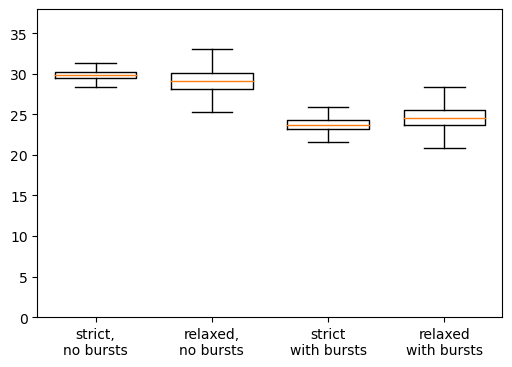
\includegraphics[width=\textwidth]{supplement/analysis/austronesian_replacement.png}
    \caption{Austronesian}
  \end{subfigure}
  \begin{subfigure}{0.4\textwidth}
    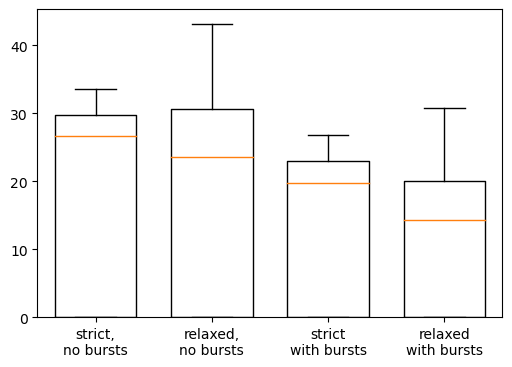
\includegraphics[width=\textwidth]{supplement/analysis/bantu_replacement.png}
    \caption{Bantu}
  \end{subfigure}
  \begin{subfigure}{0.4\textwidth}
    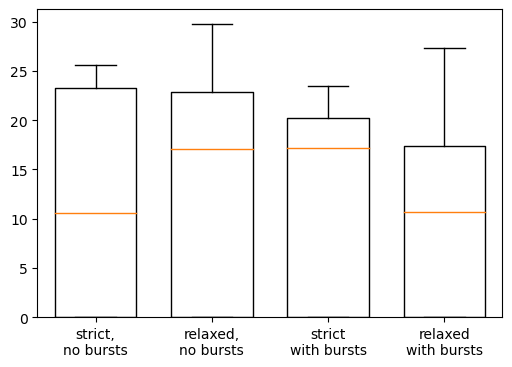
\includegraphics[width=\textwidth]{supplement/analysis/indoeuropean_replacement.png}
    \caption{Indoeuropean}
  \end{subfigure}
  \begin{subfigure}{0.4\textwidth}
    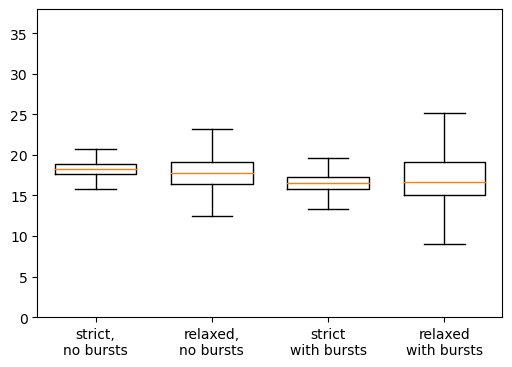
\includegraphics[width=\textwidth]{supplement/analysis/sinotibetan_replacement.png}
    \caption{Sinotibetan}
  \end{subfigure}
  \caption{Expected lexical replacement in 1000~years for the different models
    in the different language families}
    \label{f:clock}
\end{figure}

The expected lexical replacement over 1000 years according to the different
inferences is shown in \cref{f:clock}. These values are derived from the loss
rate (transition rate from ‘presence’ to ‘absence’ of a cognate class in a
concept) which governs the clock rate of the inference. While the median of our
prior lies around 44\% lexical replacement over 1000 years, the data suggests
much faster replacement, closer to \parencite{swadesh1955greater}'s
rule-of-thumb of 20\% over 1000 years, but varying widely around it, with
Austronesian showing much faster change and Sinotibetan much slower. With the
exception of Sinotibetan, the relaxed clock with bursts infers the lowest
lexical replacement rates and the strict clock without bursts the highest rates.
Because the bursts are not contributing to this estimate, they compensate for
the lower rate of change; so it is surprising that this is not seen for
Sinotibetan.

\begin{figure}
  \centering
  \begin{subfigure}{0.4\textwidth}
    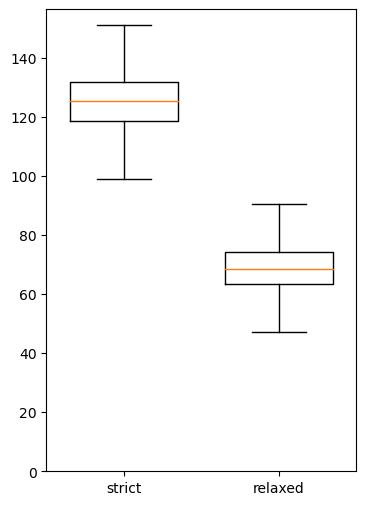
\includegraphics[width=\textwidth]{supplement/analysis/austronesian_years_per_split.png}
    \caption{Austronesian}
  \end{subfigure}
  \begin{subfigure}{0.4\textwidth}
    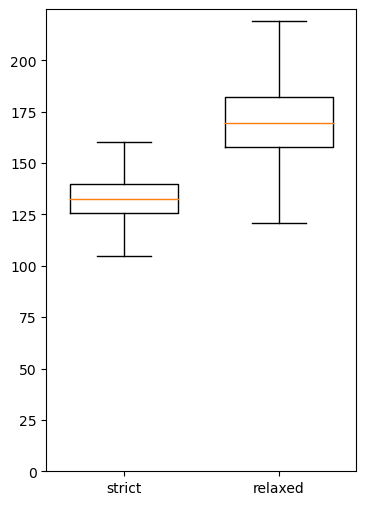
\includegraphics[width=\textwidth]{supplement/analysis/bantu_years_per_split.png}
    \caption{Bantu}
  \end{subfigure}
  \begin{subfigure}{0.4\textwidth}
    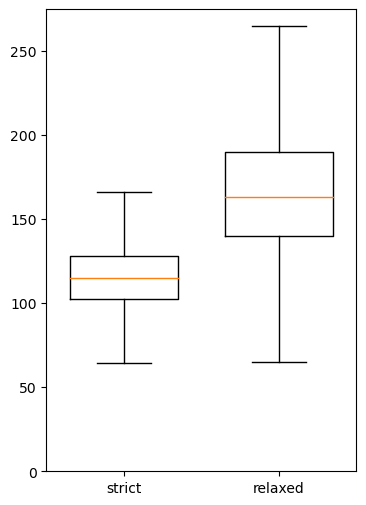
\includegraphics[width=\textwidth]{supplement/analysis/indoeuropean_years_per_split.png}
    \caption{Indoeuropean}
  \end{subfigure}
  \begin{subfigure}{0.4\textwidth}
    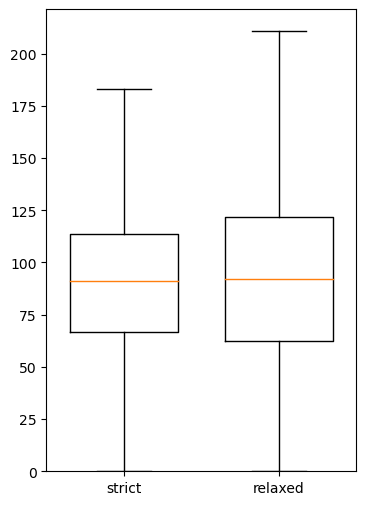
\includegraphics[width=\textwidth]{supplement/analysis/sinotibetan_years_per_split.png}
    \caption{Sinotibetan}
  \end{subfigure}
  \caption{Evolutionary contribution of each language split, in effective years}
  \label{f:peryear}
\end{figure}

The average contribution of a language split varies between $...$ and $...$
expected changes per cognate class. Comparing this with the clock rate, we get
that around the time of a split, languages change about as much as otherwise in
about 100 to 150 years of independent evolution. The distributions of the
evolutionary contributions of split events compared to time of independent
evolution in shown in \cref{f:peryear}.

In each burst clock run, the model was unconstrained and permitted to instead
select a model without bursts. The prior probability mass was equally distributed
between no bursts and bursts. Despite this prior, all samples of the
Austronesian, Bantu, and Indoeuropean analysis have a positive value for bursts,
so the Bayes factor in favour of the burst clock is the effective sample size of
the burst parameter in these models (between $...$ and $...$). For Sinotibetan,
the posterior probability of the Burst clock is $...$ as much as the clock
without bursts.

The complete setup (data, tools to generate the Beast XMLs, Beast XML files, and
run log files including tree posterior samples) is available in the
supplementary material.

\section{Discussion}
The burst clock is the preferred model. By far.

Not only is the burst clock the preferred model, but it can also contribute to
better mixing. (No guarantee!)

On the topic of mixing, what's the problem with those relaxed clocks? Did we do
something wrong, or should this cast doubt on many studies using relaxed clocks?

Our literate programming template is nice, we encourage other researchers to
adapt it, criticise it, and modify it, feeding changes back to us, so that the
field can get towards comparable studies. By the way, we think that comparable
studies across different language families haven't been done very often –
Gerhard Jäger's typological models have a similar philosophy, but if I remember
correctly, he uses existing posterior samples and builds a cross-family
hierarchical model on top of them. (Whereas our models don't inform each other,
a hierarchical model might be interesting.)

Sinotibetan is weird. The results may be due to the much stricter data coding by
the authors, or is it down to the structure of calibrations or something
actually interesting about the language family

Three explanations have been suggested for the phenomenon of schismogenesis:
Founding Effects, deliberate/conscious schismogenesis,
correlation of split rate with evolution rate. How
to distinguish them in the future?

Niche selection in Biology, like in that other paper we found recently.
(https://academic.oup.com/sysbio/advance-article/doi/10.1093/sysbio/syab085/6407161)

Random walks (diversification causing/caused by migration?) \parencite{neureitercan}

\printbibliography{}


\end{document}

% Local Variables:
% TeX-engine: luatex
% TeX-command-extra-options: "-shell-escape"
% End:
